\chapter{Efficient methods to visualize finite element meshes}
\label{chapter:mesh-visualization}

Here follows the description of the methods to process and visualize large finite element meshes. The objectives for the implementation are high responsivness, comfort of use, and low memory consumption of the final mesh editor. This text with more details is also published in \cite{Benes2015}.

%----------------------------------------------------------------------------------------
%	SECTION Theoretical background
%----------------------------------------------------------------------------------------

\section{Theoretical background}

It is needed to have the model of the problem domain as a composition of individual entities, their geometry and topological connections, before a finite element mesh is generated. The model is described by its boundary and the problem domain must be discretized for further use. This process is called mesh generation \cite{Frey2000, Rypl1998}. The output of a mesh generator is a finite element mesh corresponding to the input domain. The elements are the basic components and there are several types of them. The frequently used tetrahedral elements consist of four triangular faces described by three edges with the edge is made of two nodes.

It is sufficient to have only the list of nodes with their coordinates and the list of elements with references to their respective nodes for the mesh representation. Other entities (e.g. faces, edges) are usually omitted from the mesh generator output. However, the mesh editor has to handle them all, therefore, they must be created while loading the mesh. It is necessary to know all the kinds of the meshes that can be used as an input for the mesh editor implementation and especially for the design of the internal mesh representation. Meshes can be divided into several groups according to different criteria. The mesh classification is described in \cite{Hoppe1996}. The most basic form of mesh classification is based upon the connectivity of the mesh: structured or unstructured.

\textbf{A structured mesh}, also known as a grid, has a regular internal structure. Elements in the mesh are simply addressable due to the uniform distances between nodes. It restricts the element choices to quadrilateral in 2D or hexahedra in 3D. The regularity of the connectivity allows us to conserve space since neighborhood relationships are defined by the storage arrangement.

\textbf{An unstructured mesh} is characterized by irregular connectivity. It allows for any possible element that a solver might be able to use. When compared to the structured meshes, the storage requirements for an unstructured mesh can be substantially larger since the neighborhood connectivity must be explicitly stored.

Other mesh classification is based upon the \textbf{dimension} and the type of elements present. Depending upon the analysis type and solver requirements, meshes can be composed of one-, two- or three-dimensional elements. \textbf{Homogenous} meshes contain elements of the same type and dimension. \textbf{Hybrid} meshes are composed of elements of different type and/or dimension, e.g. tetrahedral mesh with 1D bars.

Additional classification can be made upon whether the mesh is \textbf{conformal} or not. An intersection of any two elements is either by a face, an edge or a node in conformal mesh. A non-conformal mesh contains for instance two quadrilaterals sharing two edges or two quadrilaterals sharing only a half of one edge. Non-conformal meshes are usually created during distributed generation of meshes from sub-domains and can cause issues during creation of the surface representation of non-conformal meshes. This issue is described in detail in section \ref{sec:A-implementation}.

Three-dimensional meshes can be replaced for the purpose of visualization with its surface representation. The elements (or parts of elements) that are hidden inside the volume of the mesh can be omitted. Visualization is much more efficient then. Most of the operations on entities, such as selection or setting of properties, can also be made on the mesh surface. The implementation of cuts through the volume is a problem. In order to show the entities on the cross-section, the surface representation must be regenerated each time. Making a cut is therefore a little more computationally intensive but it is outweighed by the fact that 2D surface representation is sufficient to handle any finite element mesh.

Because of the fact that the surface of both two-dimensional and three-dimensional elements is formed by either a triangle or a quadrilateral to represent the whole mesh, it is sufficient to use these two shapes. The surface representation must also include edges and vertices which the faces are formed of. The one-dimensional elements will be dealt with separately. When considering the internal representation of a mesh it is necessary to take into account the memory requirements. It should be noted that closed 3D mesh (not counting boundary elements) with homogenous structure and with $n$ elements has approximately $6n$ edges, $10n$ faces and $5n$ tetrahedral elements.

Most of the triangles and the edges will be inside the volume and can be therefore discarded after surface generation. The number of the surface entities is closely related to the geometrical shape of the domain. However, the number is significantly lower than the number of all entities for most meshes. The common operations on the mesh, e.g. to find neighboring faces, need complete topological data about the original mesh. The input file usually does not contain information about connections between elements. Therefore it must be determined while loading the mesh from the input file.

The data structure called \textbf{Winged edge} is used to store this kind of information. It is a widely used data structure in computer graphics especially for modeling practice, \cite{Baumgart1972,Floriani2004,Shirley2009}. It describes explicitly the geometry and topology of faces and allows fast traversing between faces, edges and vertices on the surface through a structure similar to the linked list. Traditional winged-edge data structure is represented by edge table. Each entry in the edge table contains these references: start vertex and end vertex, left face and right face, the predecessor and successor edges when traversing its left face, and the predecessor and successor edges when traversing its right face. Clockwise ordering (viewing from outside of the polyhedron) is used for traverse. Note that if the direction of the edge is changed, all entries in the table must be changed accordingly. Also, if some faces of a solid have holes, the above form of winged-edge data structure does not work. To make it work, ordering of the edges must be changed or some auxiliary edges must be added to surface representation. All these changes are difficult to implement efficiently. And this type of winged-edge data structure cannot be used for non-conformal finite element meshes. The basic composition of the winged-edge data structure that describes polygon meshes is widely used in computer graphics. However, the increased memory requirements compared to representations like the simple list of vertices and elements is the disadvantage. Moreover, the winged edge structure is based on dynamically created objects and therefore fragmentation of the memory can occur.

Figure \ref{fig:winged-edge} shows the adjusted data structure describing mesh surface based on traditional winged-edge schema, but eliminating some of its deficits. This structure is more suitable to use in finite element mesh scenario.

\begin{figure}[H]
\centering
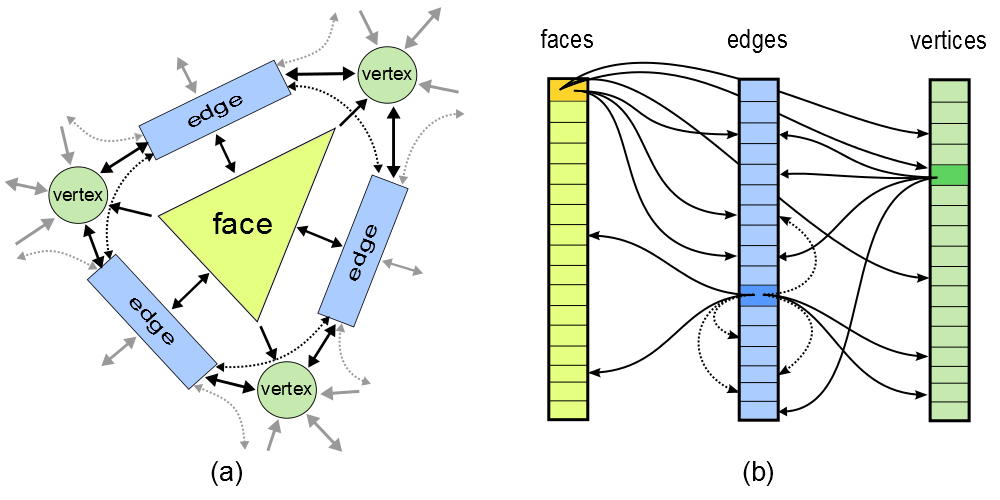
\includegraphics[width=\textwidth]{figures/chapter-mesh-visualization/figure1}
\decoRule
\caption[Winged edge data structure]{Winged edge data structure. (a) Entity dependencies. (b) Storage in lists with references.}
\label{fig:winged-edge}
\end{figure}


%----------------------------------------------------------------------------------------
%	SECTION Implementation details
%----------------------------------------------------------------------------------------

\section{Implementation details}
\label{sec:A-implementation}

All types of elements that are handled by the program are represented by the class hierarchy depicted in Figure \ref{fig:class-diagram-elements}. The common properties of all elements are accommodated in an abstract base class Element. The next level of the abstraction classifies the elements according to their spatial dimension. The particular class Beam stands for the one-dimensional element with linear approximation. The class inheriting from the Beam gains quadratic approximation by adding extra node in the middle of the line. The approximation type of other elements is distinguished by the type of their edges (a data structure describing the edge is similar to the one for 1D-elements).

\begin{figure}[H]
\centering
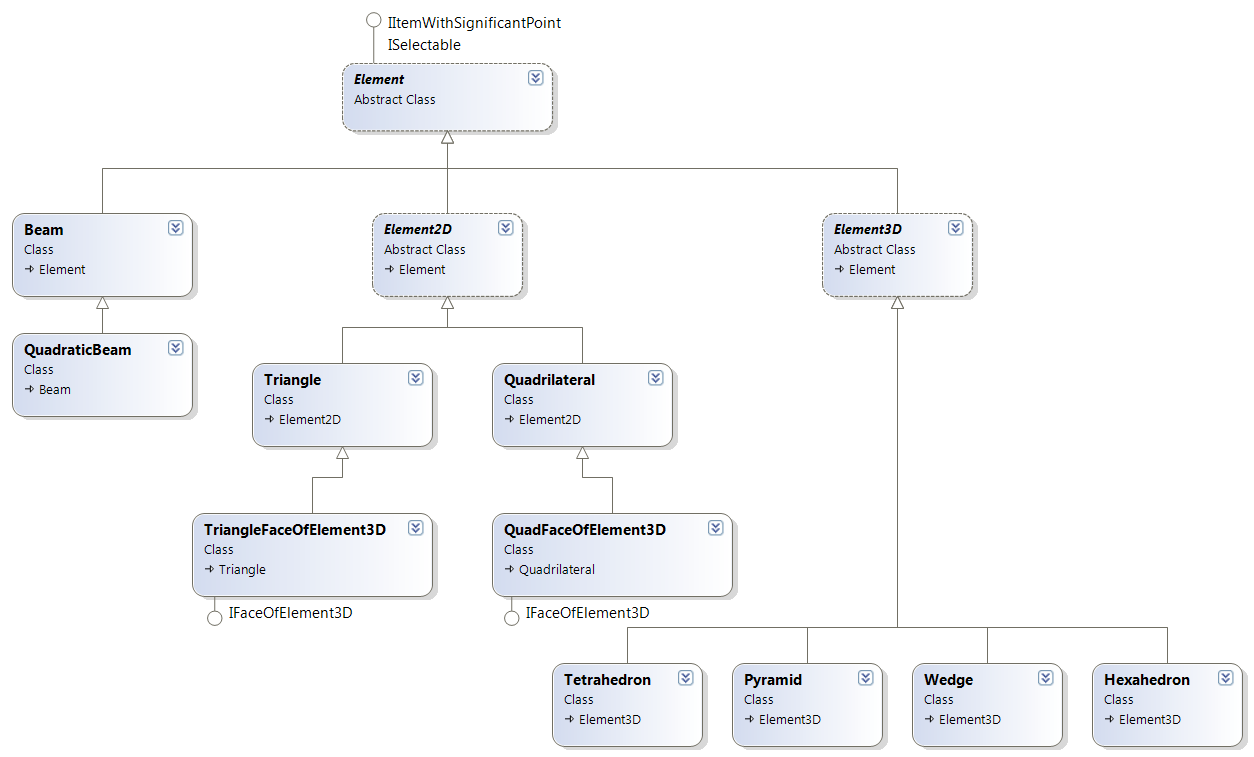
\includegraphics[width=\textwidth]{figures/chapter-mesh-visualization/figure2}
\decoRule
\caption[Class diagram of element types]{Class diagram with hierarchy of all supported element types.}
\label{fig:class-diagram-elements}
\end{figure}

The abstract base class Element2D is common for both the two-dimensional elements (triangle and quadrilateral) and faces of the three-dimensional elements (also triangles or quadrilaterals for all the widely used element types). The fact that 2D elements and faces of 3D elements can be handled in the same way allows us to implement a single generic algorithm for generation of the surface of the mesh so that the problem with hybrid meshes is hereby elegantly solved.

The 3D element face classes differ only by implementation of the interface \code{IFaceOfElement3D}.

\begin{lstlisting}
interface IFaceOfElement3D
{
	Element3D ParentElement { get; }
}
\end{lstlisting}

The interface helps to include reference to the parent 3D element at each face. This link is important for selection of elements on the mesh surface, because surface is composed, among other things, of external faces of those 3D elements that lie on the domain boundary. The adapted winged edge pattern is applied for the surface representation. All classes participating in this data structure are summarized in the class diagram in Figure \ref{fig:class-diagram-surface}.

\begin{figure}[H]
\centering
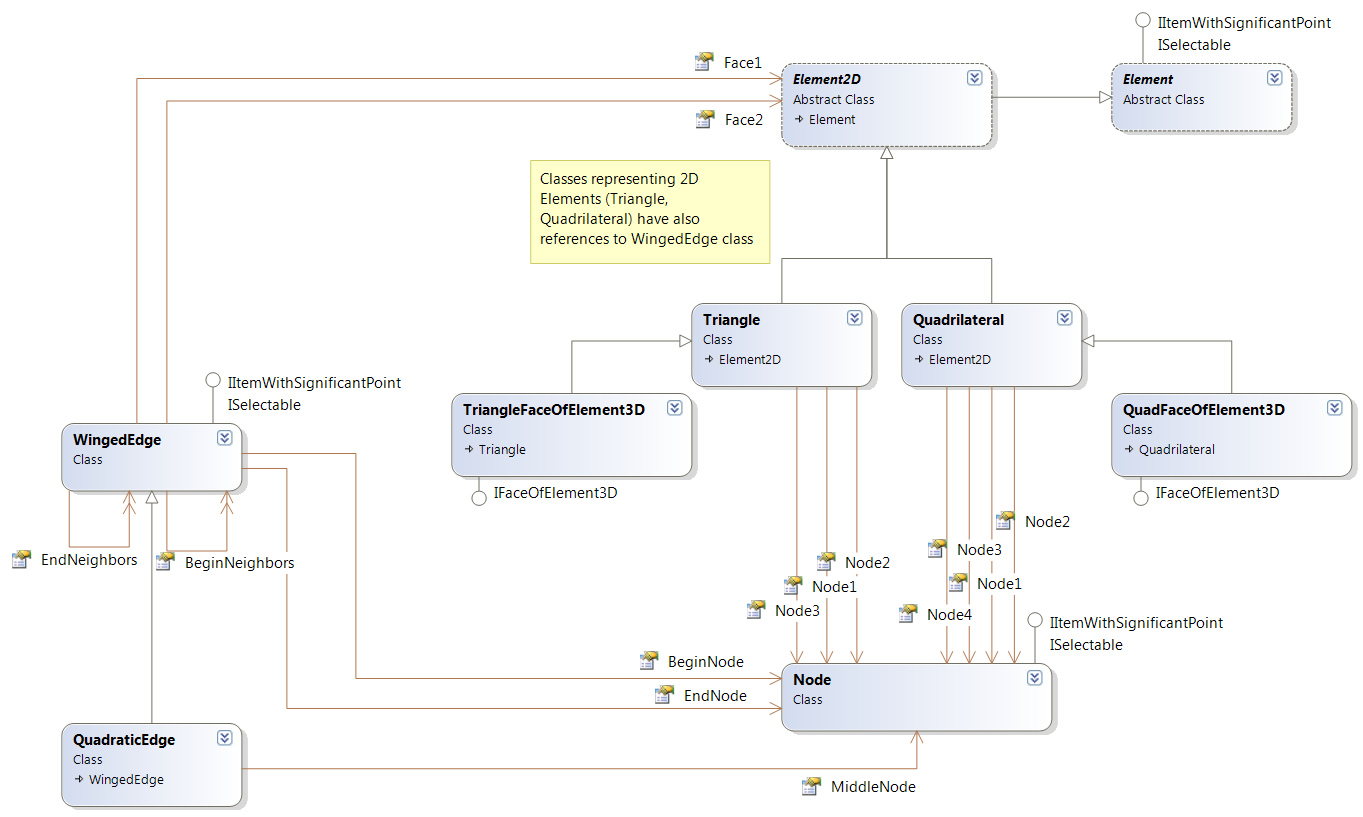
\includegraphics[width=\textwidth]{figures/chapter-mesh-visualization/figure3}
\decoRule
\caption[Class diagram of surface representation]{Class diagram with mesh surface representation.}
\label{fig:class-diagram-surface}
\end{figure}

Unlike traditional winged-edge data structure used in computer graphics in which each edge has references only to two neighboring edges, in our data structure each edge knows all its incident edges. The list of adjacent edges is tracked by every node and is shared between the node and all its neighboring edges. The ordering of edges in the list is arbitrary because in some cases there can be multiple candidates for its predecessors and successors. In this case no right ordering exists and traditional winged edge data structure used in computer graphics cannot be used. The surface representation is constructed on the fly in our single-pass algorithm. During the construction it cannot be known which edges are on the surface and what are its predecessors and successors. Therefore all adjacent edges for each node are kept in single unsorted list. To determine ordering of edges there would have to be second pass which would have significant negative impact on performance and therefore we wanted to avoid it. Moreover, for non-conform meshes there can be found no right ordering even after the surface construction.

Additionally, our approach has better memory footprint due to sharing adjacency list between node and all its neighboring edges as oppose to traditional winged edge structure. Another advantage is better performance in most common use cases of the mesh editor. Every user-triggered operation with mesh starts with selection of node or face on the mesh surface. Having direct references between each node and all its incident edges enables us quickly traverse the whole mesh surface.

Another adjustment of our data representation that differs from winged edge structure used in computer graphics is calculating and storing angle between each two neighboring faces. This enables us to implement advanced features such as finding significant edges or selection of logically related elements (e.g. on the same flat surface) as described below.

Besides the references to the begin- and end- nodes, every edge also has references to the lists of neighboring edges for each of both nodes. The lists are shared between the adjacent edges to achieve lower memory consumption. The edge also contains references to the faces on the left and on the right. This kind of linking is suitable for the majority of meshes. A problem can occur only in the non-conformal mesh processing when elements can share only a part of its surface. Visualization of this mesh can show up some artifacts caused by the fact that some internal faces do not have the adjacent counterparts and thus cannot be paired off. Another problem shows up when some elements have only one edge in common. In that case, the edge can be shared by more than two faces and the winged edge data structure cannot capture properly this situation. However, these are rare cases and do not render the program unusable.

%----------------------------------------------------------------------------------------
%	SUB-SECTION Data structures overview
%----------------------------------------------------------------------------------------

\subsection{Data structures overview}

The modified winged-edge data structure was used to describe the internal surface representation of a mesh. Instead of references to the left and the right adjacent edges, each node has reference to the list of all edges that begin or end at this node. The references to these lists are also contained in each winged-edge object. This approach allows representing the meshes with some abnormalities or non-conformal meshes in where it is impossible to determine which edge is the left and which is the right. Other characteristics of the winged-edge data structure remain the same. Each edge has references to the left and the right adjacent faces. Each face has references to its nodes, edges and the parent 3D element. The elements need to have references only to its nodes, because not every element is on the mesh boundary and so it does not need to have reference to surface objects. Every operation on the mesh, such as selection, begins with either a face or a node on the surface. Other entities are found by searching through the links in the winged edge data structure. Figure \ref{fig:data-structure-mesh} shows data lists used in the mesh editor.

\begin{figure}[H]
\centering
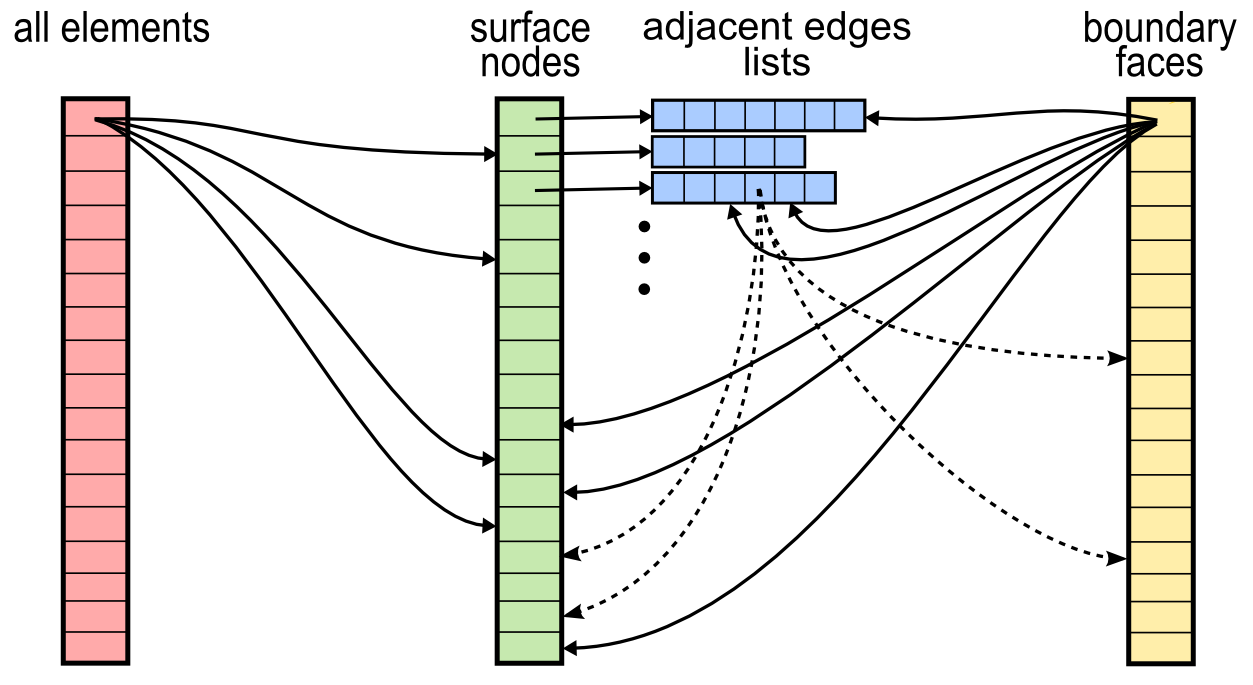
\includegraphics[width=\textwidth]{figures/chapter-mesh-visualization/figure4}
\decoRule
\caption[Data structure overview]{Diagram with data structure overview.}
\label{fig:data-structure-mesh}
\end{figure}

Memory requirements of each entity object are summarized in Figure \ref{fig:surface-rep-memory}. The overall memory consumption depends highly on the mesh topology and on the ratio of the number of surface elements to the total number of elements. This ratio decreases with the growing size of the mesh (or the element density) because the total number of elements increases with cube of the size of mesh, unlike the number of surface elements which increases with square of the mesh size.

\begin{figure}[H]
\centering
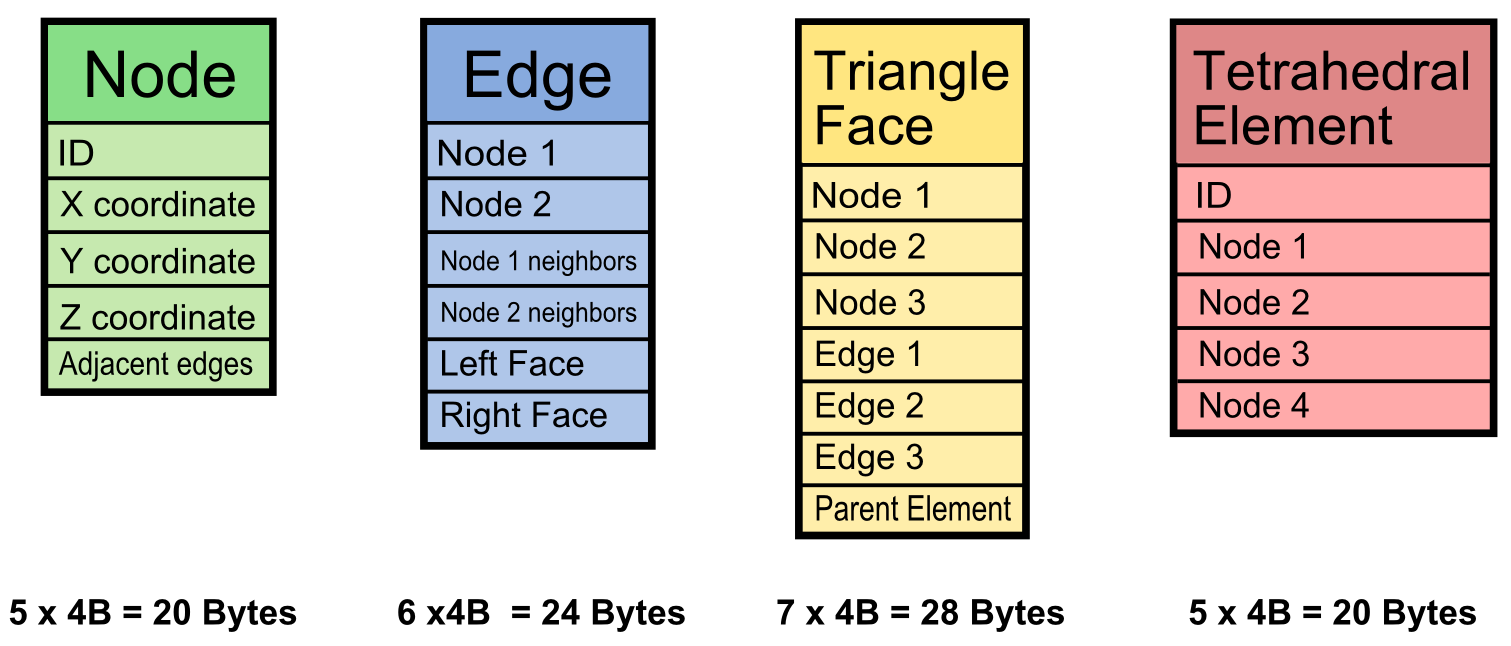
\includegraphics[width=\textwidth]{figures/chapter-mesh-visualization/figure5}
\decoRule
\caption{Memory consumption of the surface representation.}
\label{fig:surface-rep-memory}
\end{figure}

%----------------------------------------------------------------------------------------
%	SUB-SECTION Surface representation construction
%----------------------------------------------------------------------------------------

\subsection{Surface representation construction}

The process of creating the mesh surface representation is the key feature. It was designed as a one-pass algorithm which finds surface entities and creates the winged edge data structure on the fly during loading an input file. It should be noted that the input file does not contain any relationships between the mesh entities besides the coordinates of each node and a simple list of elements with links to relevant nodes.

The main problem is to find those faces of 3D elements that belong to the mesh surface. To resolve this issue we started with the consideration that each internal face has its twin in the adjacent element. While loading each element from the file, all its faces are generated. Then, the faces are included to a global hash table \cite{Knuth1998}. The key to this table is a special object consisting of the face node IDs. If the face under same key already exists, it means that the face is an internal face that we do not consider. Hence, the face is thrown away and the twin face is removed from the hash table. The procedure is repeated until all faces of all elements are processed. At the end (for conformal meshes) it is guaranteed that all remaining faces in the table are on the mesh boundary. For non-conformal meshes the algorithm can produce also some internal faces. Additional check for these situations is possible but it would break the simplicity and performance of the algorithm. Figure \ref{fig:mesh-construction} shows a diagram with the progress of loading an input file and constructing the mesh internal representation.

\begin{figure}[H]
\centering
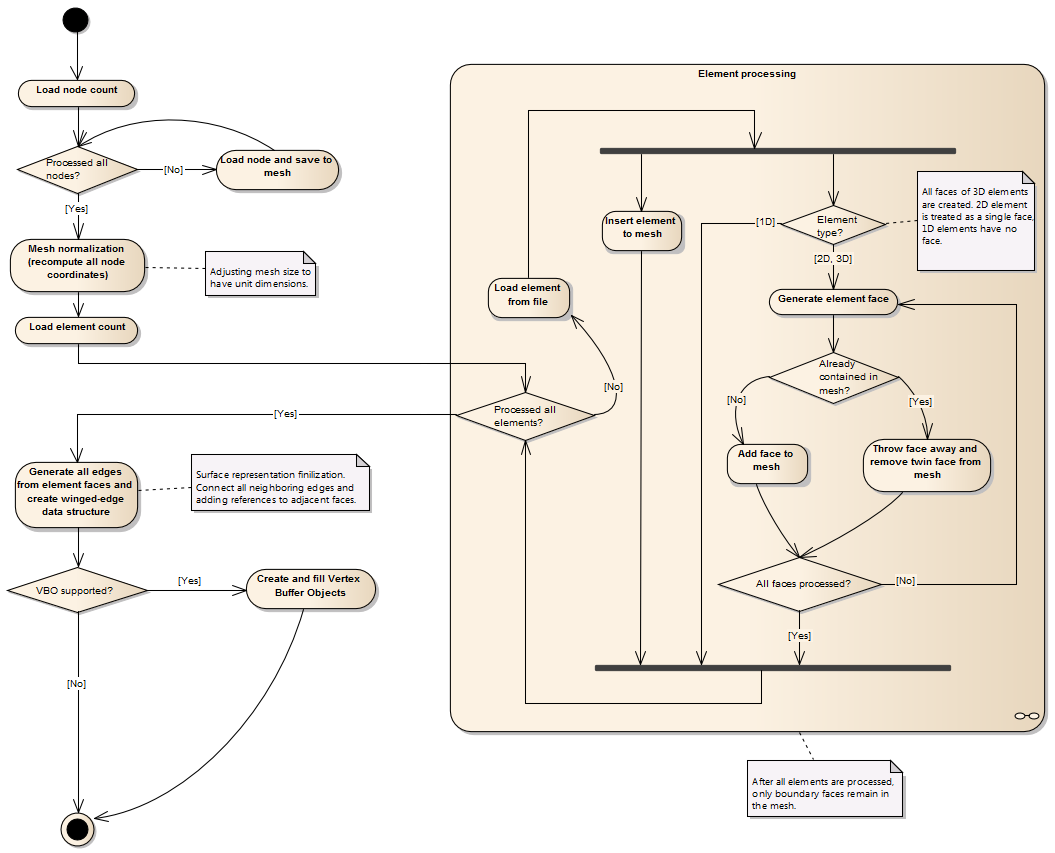
\includegraphics[width=\textwidth]{figures/chapter-mesh-visualization/figure6}
\decoRule
\caption[Activity diagram of mesh construction]{Activity diagram of loading and construction mesh surface representation.}
\label{fig:mesh-construction}
\end{figure}

In order to complete the surface representation, the edges must be generated from their faces. The analogous procedure that works with the hash table of edges is used here. Each edge has its twin in the adjacent face on the surface. But only one representative is needed. If a new edge is included into the table and under the same key the object is already contained, the new edge is thrown away. But compared to the previous case the edge in the table is not removed. The byproduct of this algorithm is finding the edges on the surface boundary. These edges have no twins as they have only one neighboring face. This however applies only to two-dimensional meshes, since the 3D meshes have a closed boundary.

Finally, when all surface entities are found, the Vertex Buffer Object (VBO) is created. It is an OpenGL feature that provides methods for uploading vertex data to the video device for rendering. VBO offers substantial performance gains over the immediate mode rendering because the data resides in the video device memory rather than the system memory and so it can be rendered directly by the video device. However, the buffer of rendered data must be updated each time the surface geometry changes. All up-to-date video cards support the VBO feature. If the card still does not support this feature, the application is smart enough to use the immediate-mode for rendering.

%----------------------------------------------------------------------------------------
%	SUB-SECTION Looking inside the mesh
%----------------------------------------------------------------------------------------

\subsection{Looking inside the mesh}

The editor allows to hide (or delete) some group of elements to enable the user to look inside the mesh. This makes sense especially for the 3D models when the user wants to see and manipulate the internal entities. Let us suppose that the set of elements to be hidden is known. Firstly, the program disposes of the current mesh surface representation and after that it basically creates the entire surface again with the use of the above mentioned effective surface representation construction algorithm. However, in this case the algorithm does not take all the elements from the input file as an input parameter, it take only those that are \textbf{not} contained in the list of elements to be removed. This solution offers the possibility to reuse the existing code that is already optimized and universally applicable to all types of meshes.

Moreover, this approach simplifies the implementation of other useful features summarized in the following list (all the features use the same surface construction algorithm).

\begin{itemize}
	\item \textbf{Hide selected elements} -- remove a set of arbitrary elements selected by the mouse pointer.
	\item \textbf{Show or hide elements with specific property} -- e.g. turn on or off layers containing elements with the same material id.
	\item \textbf{Cut through the mesh defined by plane} -- hide all the elements that are located behind the plane specified with three points lying in the plane or by a point on the plane and a normal vector. In this case only the elements that fall entirely behind the cut plane are displayed. Then the view is not perfect, but this approach is needed in our editor, where we have to assign properties to individual entities such as nodes and faces of elements. If the cut portion of the elements intersecting the cut plane would be displayed, editing of entities on the cut will not be possible. Also the implementation would be more complicated and our winged-edge data structure could not be used.
	\item \textbf{Cut through the mesh defined by general algebraic equation} -- previous operation (cut defined by plane) uses internal testing function that takes the point coordinates as an input parameter and returns a boolean value saying whether the point lies inside the area to be removed or not. The testing function is called for all currently visible elements. The testing function is in this case generalized to test the point against the algebraic equation specified by the user.
\end{itemize}

Each time the cut is performed the surface representation of the mesh is regenerated. Therefore turning on the cuts has no effect on the speed of manipulating views. All calculations are performed only during applying the cut through the mesh.

%----------------------------------------------------------------------------------------
%	SUB-SECTION Finding visible nodes
%----------------------------------------------------------------------------------------

\subsection{Finding visible nodes}

For various operations with a mesh, it is useful to have some method that finds the set of nodes that are visible from the current view-point, i.e. nodes that are not hidden behind a part of the mesh. Apart from the rendering of nodes and labels on the mesh surface, information about visible nodes can be used for implementation of the method for selection of entities on the surface using the mouse pointer.

The principle of the method is simple. Firstly, the method performs the perspective projection of all nodes to the screen and their actual depth is determined. Then the whole model is rendered into depth-buffer to produce a depth-map of the mesh. After that, the value in the depth-buffer corresponding to each node is compared to the Z-component of the screen coordinates of this node. If the value in the depth-buffer is greater than the projected distance of the node, the node is hidden behind some face. Otherwise, the node is added to the visible nodes set. The best precision in the depth-buffer is for the vertices that are in a small distance from the front clipping plane of the viewing frustum. The first step of the algorithm is therefore to move the near clipping plane from the observer to the mesh surface as close as possible. The pseudo-code of the described algorithm follows.

\begin{lstlisting}
Set<Node> FindVisibleNodes(Rectangle area)
{
	GL.MatrixMode(MatrixMode.Projection);
	GL.LoadIdentity();
	// move the Near plane closer to model for better precision
	double newZ_NEAR_PARAM = ComputeMeshMinVisibleDistance();
	// set perspective projection with updated parameters
	Glu.Perspective(FOVY_PARAM, aspect_ratio, newZ_NEAR_PARAM, Z_FAR_PARAM);
	// ---------------------------------------------------------------------
	// compute projections of all nodes to screen coordinates
	Dictionary<Node, Vector3> projections = new Dictionary<Node, Vector3>();
	Vector3 winPos;
	foreach (Node node in allSurfaceNodes)
	{
		Glu.Project(node.Position, modelview, projection, viewport, out winPos);
		if (area.Contains(winPos.X, winPos.Y)) // if the point is inside area,
			projections[node] = winPos;  // save projection to dictionary
	}
	// ---------------------------------------------------------------------
	// draw faces to depth buffer
	GL.Clear(ClearBufferMask.DepthBufferBit);
	GL.PolygonOffset(1f, 1f); // move little bit to enable testing
	GL.Enable(EnableCap.PolygonOffsetFill);
	DrawFaces();
	GL.Disable(EnableCap.PolygonOffsetFill);
	// ---------------------------------------------------------------------
	Set<Node> result = new Set<Node>();
	foreach (KeyValuePair<Node, Vector3> pair in projections)
	{
		Node node = pair.Key; winPos = pair.Value; float pixelDepth;
		GL.ReadPixels(winPos.X, winPos.Y, 1, 1, Format.Depth, Type.Float, out pixelDepth);
		// !! key depth test; if passes, node is visible
		if (winPos.Z <= pixelDepth)
			result.Add(node);
	}
	return result; // return list of visible nodes
}
\end{lstlisting}

%----------------------------------------------------------------------------------------
%	SUB-SECTION Selection of entities
%----------------------------------------------------------------------------------------

\subsection{Selection of entities}

The mesh editor implements a tool for selection of entities in the mesh. The tool has two modes. The first mode allows user to select entities contained in the rectangular area specified by dragging the mouse pointer. Implementation of this tool uses the above mentioned method \code{FindVisibleNodes()}. The set of nodes returned by the method is then transformed to the set of entities that the user wants to select by looking to the winged edge data structure that takes advantage of its rich interconnections. For example, if the user wants to select all the edges in the rectangular area, the algorithm finds all edges that have one of theirs node in the set of nodes returned by the method \code{FindVisibleNodes()} that takes the selection rectangle as a parameter.

The second mode of the tool is selection of some geometrically related entities, e.g. all nodes on the top of the mesh. The input file that is used does not contain any information about neither the model from which the mesh was generated nor the curves and planes that form the surface of the model. However, the user usually requests to be able to select such groups of entities.

The core of the implementation of this functionality is the method \code{SelectSurface()}. The method returns the set of element faces on the mesh surface that have pre-specified maximum angle between them. The angle (passed as a function parameter) defines the degree of smoothness of the resulting surface.

The limit angle is determined by the count of the mouse button clicks on some face. The target face is also passed as an input parameter of the function. The limit angle increases with a growing number of clicks. The program operates with four levels of tolerance in the surface selection. The default values of the limit angles for each level are carefully chosen to suit the largest number of the mesh. For atypical-formed meshes, the user can change these default parameters.

The following pseudo-code shows the implementation of the \code{SelectSurface()} method. Figure \ref{fig:element-face-selection} illustrates the result of the double- and triple-click on the mesh surface. Double-click selects all faces in the area that is delimited by the first limit angle. Default value of this parameter is one degree. Therefore double-click selects the elements or faces of elements which have a face on the same flat surface as the mouse cursor, whereas the triple-click selects the elements or faces on the smooth (possibly curved) surface as the mouse cursor. This surface is delimited by edges whose adjacent faces include angle lower than or equal to the second limit angle. Fourth click selects all the remaining neighboring elements or faces.

\begin{lstlisting}
Set<Element2D> SelectSurface(Element2D startFace, float borderAngleLimit)
{
	Set<Element2D> selectionSet = new Set<Element2D>(); // faces to select
	Stack<Element2D> faces = new Stack<Element2D>(); // visited faces
	faces.Push(startFace); // push starting face
	selectionSet.Add(startFace);
	while (faces.Count > 0) // while the stack is not empty
	{
		Element2D face = faces.Pop();
		// add to the stack all neighboring faces
		// that form with the face an angle of value at most borderAngleLimit
		foreach (Element2D neighbor in face.GetNeighbors(borderAngleLimit))
		{
			if (!selectionSet.Contains(neighbor))
			{
				faces.Push(neighbor);
				selectionSet.Add(neighbor);
			}
		}
	}
	return selectionSet;
}
\end{lstlisting}

\begin{figure}[H]
\centering
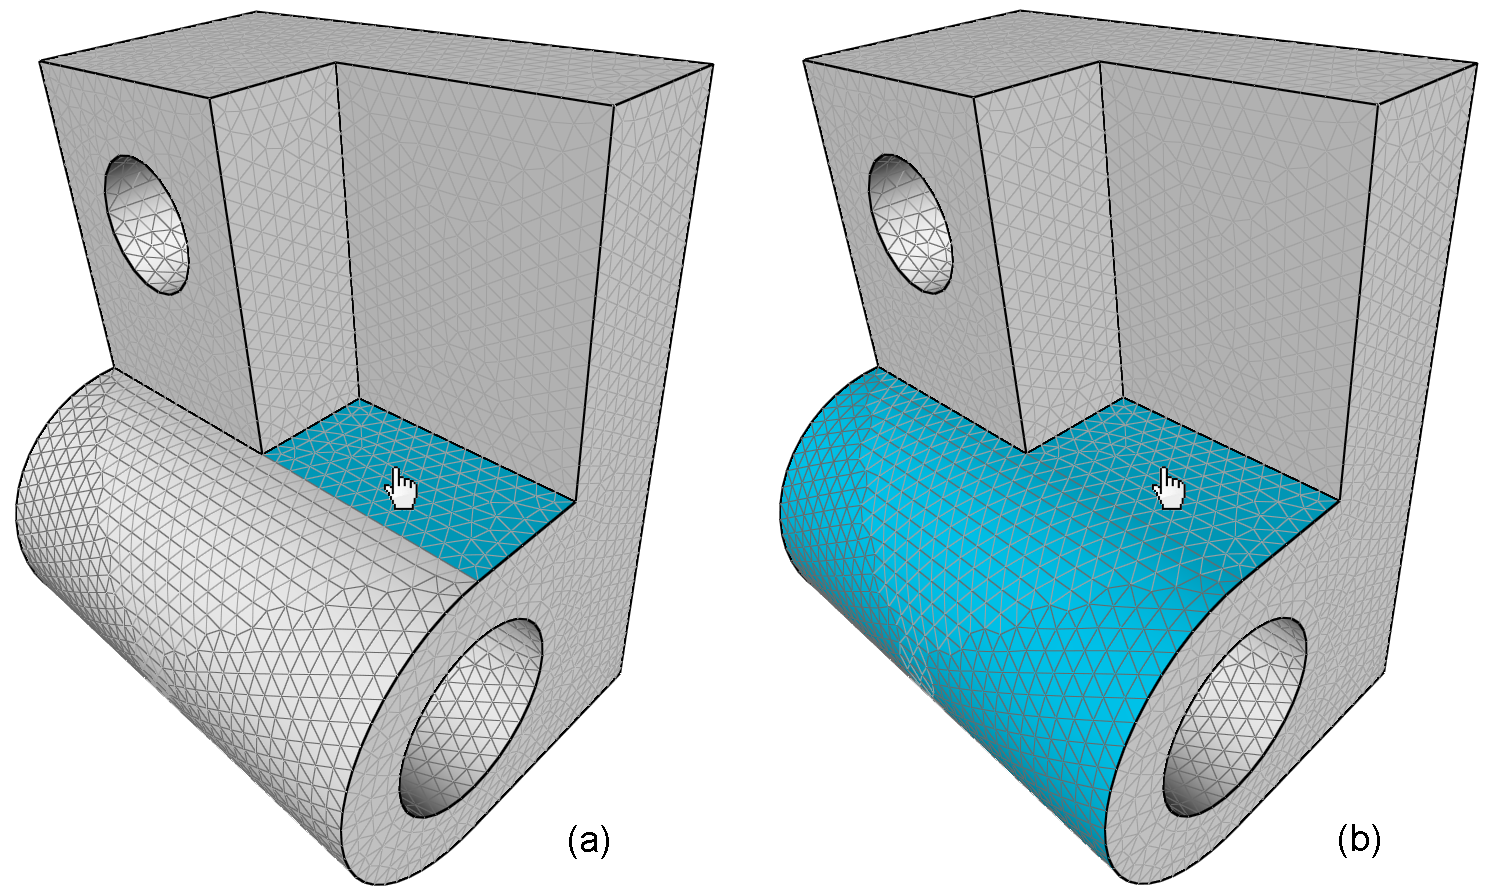
\includegraphics[width=\textwidth]{figures/chapter-mesh-visualization/figure7}
\decoRule
\caption[Selection of element faces]{Selection of element faces on the mesh surface. (a) Result after mouse double-click. (b) Result after mouse triple-click.}
\label{fig:element-face-selection}
\end{figure}


%----------------------------------------------------------------------------------------
%	SECTION Results
%----------------------------------------------------------------------------------------

\section{Results}

The program was benchmarked against other commonly used editors that have similar capabilities. We chose the \textbf{GiD} \cite{GiD2013} postprocessor, \textbf{ParaView} \cite{ParaView2005} and \textbf{VisIt} \cite{VisIt2005}. The initial loading time (see Table \ref{tab:loading-time}) and memory consumption were measured (see Table \ref{tab:memory-consumption}). The memory requirements of our mesh editor grows slightly faster than requirements of other tools for meshes with high number of finite elements. It is caused by auxiliary data structures assembled for future fast manipulation with meshes. The mesh Beam with $651.873$ elements represents a limit task which can be solvable on a single processor computer. For smaller problems, memory requirements of our editor are comparable or even smaller in comparison with GiD, ParaView and VisIt. Figure \ref{fig:benchmark-meshes} contains visualizations of the meshes that were used in the benchmark.

\begin{table}
\caption[Initial loading time comparison]{Measured results: Initial loading time in seconds (CPU time).}
\label{tab:loading-time}
\centering
\begin{tabular}{| l | r | r | r | r |}
\hline
\tabhead{mesh (size)} & \tabhead{MeshEditor} & \tabhead{GiD} & \tabhead{ParaView} & \tabhead{VisIt} \\
\hline
Beam (651873 elements) & 36 & 28 & 16 & 24\\
Beam (47680 elements) & 4 & 5 & 3 & 2\\
Beam (3222 elements) & 1 & 4 & 2 & 1\\
Sphere (348014 elements) & 4 & 3 & 7 & 2\\
Robo (244188 elements) & 7 & 7 & 7 & 7\\
\hline
\end{tabular}
\end{table}

\begin{table}
\caption[Memory consumption comparison]{Measured results: Memory consumption in megabytes (Private working set) [MB]}
\label{tab:memory-consumption}
\centering
\begin{tabular}{| l | r | r | r | r |}
\hline
\tabhead{mesh (size)} & \tabhead{MeshEditor} & \tabhead{GiD} & \tabhead{ParaView} & \tabhead{VisIt} \\
\hline
Beam (651873 elements) & 824.616 & 620.956 & 339.436 & 526.144\\
Beam (47680 elements) & 104.124 & 92.772 & 128.888 & 123.244\\
Beam (3222 elements) & 42.800 & 52.480 & 114.380 & 89.116\\
Sphere (348014 elements) & 108.324 & 106.428 & 133.652 & 128.808\\
Robo (244188 elements) & 291.836 & 200.484 & 543.316 & 355.268\\
\hline
\end{tabular}
\end{table}

\begin{figure}[H]
\centering
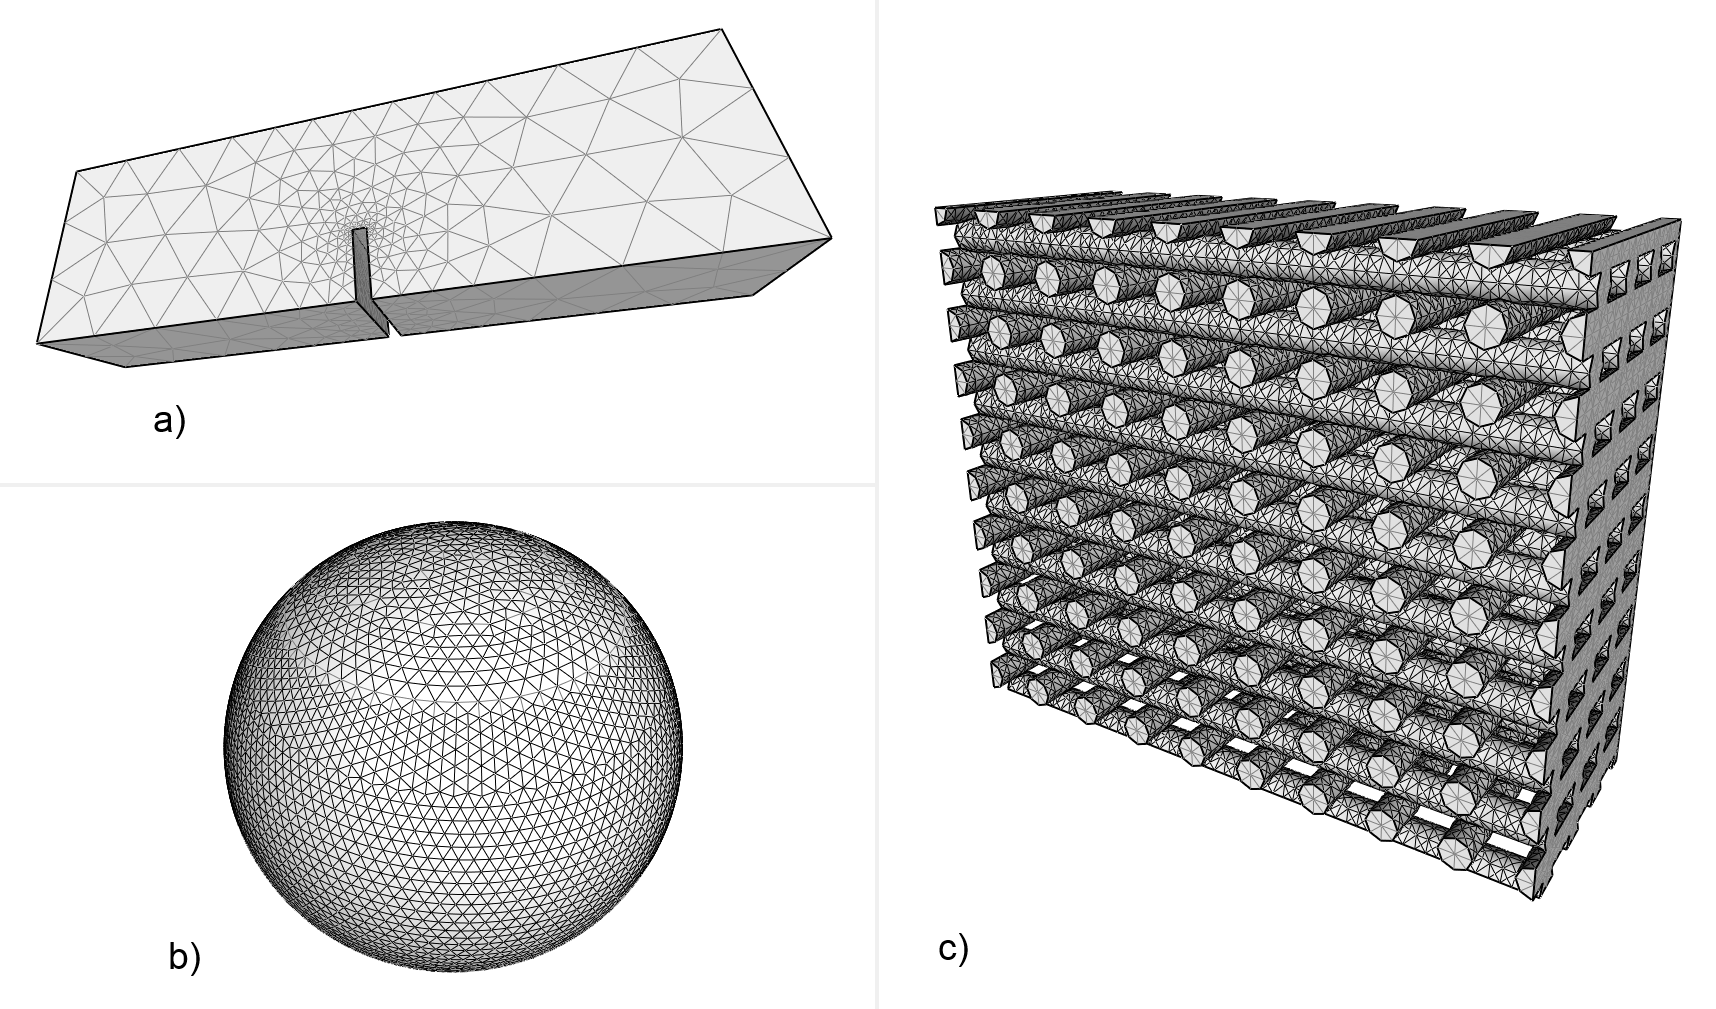
\includegraphics[width=\textwidth]{figures/chapter-mesh-visualization/figure8}
\decoRule
\caption[Meshes for benchmarks]{Visualizations of meshes used in benchmark. Three different densities of the Beam mesh were used to demonstrate the effects of mesh size. Meshes Sphere and Robo show effect of surface area/volume ratio. a) Beam. b) Sphere. c) Robo.}
\label{fig:benchmark-meshes}
\end{figure}

\begin{figure}[H]
\centering
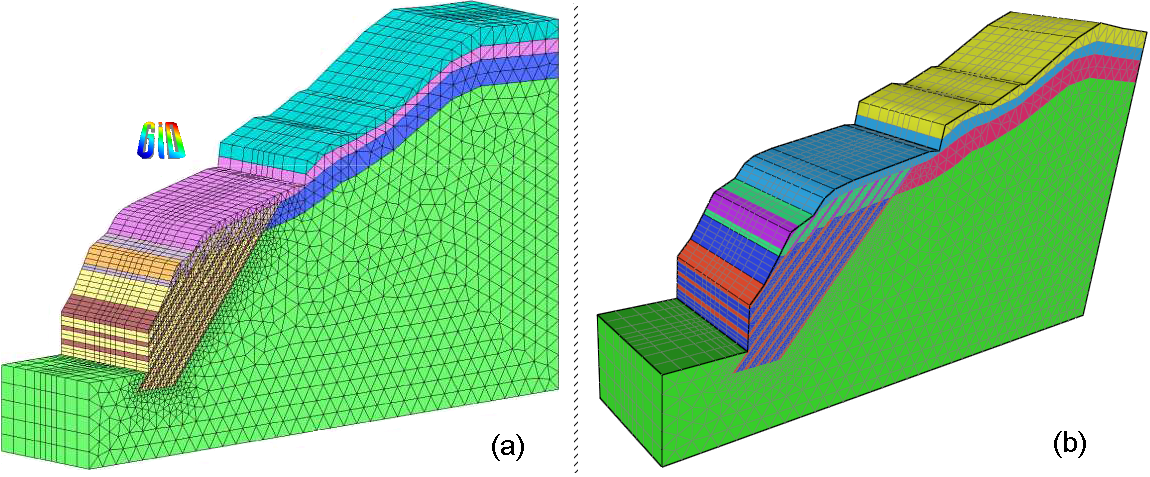
\includegraphics[width=\textwidth]{figures/chapter-mesh-visualization/figure9}
\decoRule
\caption[Visualization of significant edges]{Finding and visualization of significant edges. a) GiD postprocessor. b) The Mesh Editor.}
\label{fig:significant-edges}
\end{figure}

For benchmarking we used PC with Intel Core i7-2600 processor, 16 GB memory and NVidia GeForce GT 545 graphics card. The results support the fact, that more complex data structure is constructed to represent the mesh in our editor. The manipulation with the model is comfortable even for a very large data input. The program takes benefit of creating the sophisticated internal data structure that, on the contrary, causes longer initial loading time. However, the presented smart internal model representation allows selection of logically related groups of entities on the mesh surface without knowing the geometrical and topological connections from the modeller. The program is able to find automatically the significant edges where the geometry changes (shown in Figure \ref{fig:significant-edges}) and therefore simplify the process of selecting the entities. Moreover, individual elements can be easily removed so it is allowed to dig into the mesh and view the internal elements. The other editors, which were tested against the proposed editor, do not support those features. Besides that, the capability of unlimited view-point movement allows to fly through holes in the mesh and investigate the mesh from the inside.